\documentclass[10pt]{article}

\usepackage[utf8]{inputenc}
\usepackage[english]{babel}
\usepackage[T1]{fontenc}
\usepackage{wasysym}
\usepackage{pgfgantt}
\usepackage{pdflscape}
\usepackage{geometry}
\usepackage{url}
\usepackage{hyperref}
\usepackage{xifthen}
\usepackage{setspace}
\usepackage{pgffor}
\usepackage{graphics}

\usepackage[autostyle]{csquotes}
\usepackage[
  backend=biber,
  style=numeric,
  url=true,
  sorting=none
]{biblatex}
\bibliography{pplan}
%\usepackage{fontspec}
%\setmainfont[Ligatures=TeX]{Georgia}

\setlength{\parindent}{0cm}

\newcounter{countQuestions}
\newenvironment{question}
  {%
%    \begin{doublespacing}
  }%
  {%
%    \end{doublespacing}
  }%

\newcommand{\qmline}[2][]{%
  #2? \\ \ \\
  \ifthenelse{\isempty{#1}}%
    {\rule{\textwidth}{0.4pt} \\ \\ \rule{\textwidth}{0.4pt} \\ }%first is empty.
    {%
      \foreach \index in {1, ..., #1} {%
        \rule{\textwidth}{0.4pt} \\ \\
      }
    }%first is not empty.
    \\
}

\newcommand{\qline}[2][]{%
  \ifthenelse{\isempty{#1}}%
    {#2: }%first is empty.
    {#2 [\textit{Ex: #1}]: }%first is not empty.
    \hrulefill \\ \\
}
\newcommand{\hh}{\hspace{1cm}}
\newcommand{\qscale}[1]{%
  \textit{#1}: \\
    Strongly Disagree\ 1---2---3---4---5---6---7\ Strongly Agree
  %  \fullmoon \ Never  \hh
  %  \fullmoon \ Sometimes  \hh
  %  \fullmoon \ Most of the time  \hh
  %  \fullmoon \ Always
  \ \\ \\
}

\newcommand{\myenquote}[1]{\enquote{\itshape#1}}


\begin{document}

\begin{center}

%Projektplanering Alla större arbeten tjänar på att planeras, inte minst ett
%examensarbete som pågår ungefär ett halvår. Det kan vara en god idé att använda
%det tidigare skrivna måldokumentet som en stomme till en projektplan. I
%projektplanen beskrivs arbetets innehåll, avgränsningar och metodik relativt
%detaljerat. Detta innebär bland annat att försöka planera vilka mätningar,
%beräkningar, intervjuer eller andra undersökningar som ska utföras, och hur man
%avser att tolka och analyser de resultat som detta ger. En sådan plan kommer
%givetvis att variera högst väsentligt mellan olika examensarbeten.
%
%En annan viktig del i planeringen är upprättande av en tidsplan. För att
%underlätta styrning och uppföljning av projektet bör arbetet delas upp i mindre
%delmoment och avstämningspunkter. Det är lätt hänt att tiden rinner iväg,
%vilket i viss mån kan regleras med en tidsplan. En tidsplan ska, så bra som
%möjligt, uppskatta den tid som de olika momenten i examensarbetet kan ta. Det
%är viktigt att på ett tidigt stadium av arbetet få en uppfattning av hur mycket
%tid som finns tillgänglig för de olika delmoment som ingår. Ett examensarbete
%ska motsvara 20 veckors heltidsstudier. Begränsningen är givetvis inte strikt,
%men kan vara ett riktmärke att jobba efter. Det är viktigt att även ta hänsyn
%till konkurrerande aktiviteter såsom studentens/studentgruppens eventuella
%parallella studier och handledarens eventuella längre tjänsteresor.
%
%Det kan också vara bra att fundera över formerna för handledning på ett tidigt
%stadium, och klargöra respektive parters förväntningar på varandra. En del
%tycker att en form med regelbundna möten fungerar bra, andra trivs med att
%träffas efter behov. En projektplan ska definiera avstämningspunkter med alla
%handledare.
%
%Tänk på att inte bara planera för själva utredningsarbetet utan också ta med
%aktiviteter i slutfasen t.ex. opponering och presentation där diverse praktiska
%saker som tid för tryckning av rapporten, presentationsförberedelser och
%liknande kan påverka tidsplanen för arbetet.
%
%Planering inte är något statiskt. Många examensarbeten har karaktär av
%forskning eller utveckling, vilket innebär att man inte vet riktigt vad man har
%att vänta sig. En god planering måste vara tillräckligt flexibel för att ta
%hänsyn till detta. Projektplanen bör uppdateras löpande och förändringar bör
%diskuteras med huvudhandledaren.

  % Arbetstitel.
  Degree project \\
  \ \\
  {\large
    \textbf{Project plan for degree project}
  } \\
  %} \\
  %--- \\
  \ \\
  Stefan Eng \texttt{<atn08sen@student.lu.se>}
  \ \\
  \today \\
  \ \\
  ---
  \vspace{-0.3cm}

\end{center}

\tableofcontents

\begin{center}
---
\end{center}

\section{Project Purpose}

  The primary aim is to evaluate in what capacity, if any, theory and practical
  results gained from the fields of human-computer interaction\cite{c_hci}
  (HCI), and Cognitive science\cite{c_congnitivescience} can be used to improve
  interaction with a third party software. More specifically, the interaction
  studied will be the one between employees at Massive
  Entertainment\cite{c_massive} and the Shotgun\cite{c_shotgun} software suit.
  \\

  If there is a positive impact, the secondary objective is to try to
  quantify the benefits and weigh them against the work done. This will be done
  in order to determine if investment in and expansion of this type of tailor
  made adjustments would benefit Massive in other areas.



  %Arbetet kommer att undersöka i vilken utsträckning forsknings-resultat
  %från, samt teorier inom området människa-datorinteraktion, MDI\cite{c_mdi},
  %eller engelska motsvarigheten, HDI\cite{c_hci} kan underlätta användningen av
  %Shotgun\cite{c_shotgun} på Massive Entertainment\cite{c_massive}, Malmö.
  %Målet är främst att mäta om en skräddarsydd interaktionslösning har en
  %positiv inverkan på användareupplevelsen, och sekundärt, om den är stor nog
  %att motivera det initial arbetet.

\section{Project Restrictions}

  %Arbetet kommer främst fokusera på att analysera interaktioner med
  %Shotgun\cite{c_shotgun}, en mjukvaran som används för att skapa och hålla
  %uppsikt på utvecklingen av multimedia projekt. Vid diskussion har det framkommit
  %att det finns ytterligare system som hade varit intressanta att analysera,
  %men som ej kommer utföras på grund av begränsad tid.

  There are inherit restrictions that will apply to the project process which
  need to be addressed.

  \subsection{Scope of Evaluation}

    Massive uses many different types of software in order to coordinate and
    produce their games, and after some discussion there were several software
    candidates that could be analyzed. Since this project has a limited time
    budget of approximately 20 weeks, one candidate was chosen, Shotgun. \\

    This choice does not indicate that there are more problems with Shotgun
    than other software, but since it is a communications and project-planning
    software, increased usability of this tool in particular would benefit the
    team as a whole.

    %Målet är att identifiera mellan tre till tio ofta förekommande arbetsflöden
    %som består av minst tre distinkta handlingar som exempelvis fil-operationer
    %och mus-klick där användare upplevt irritation eller att det kan ske
    %förbättringar.

  \subsection{Number of Participants and Biases}

    In \citetitle{c_handbook_usability}\cite[p.126]{c_handbook_usability}, the
    authors recommend that in order to \myenquote{expose the vast majority of
      usability problems} a project that has three tests planned should aim at
    a group size of four to five people in each group, resulting in twelve
    to fifteen participants in total. The number of total participants is not a
    restriction in of itself, but ensuring a good mix of roles in each group
    and compensating for biases from, as an example, longer usage of Shotgun
    has to be addressed.

    %Vid tre utförda tester rekommenderas minst fyra till fem personer i varje
    %grupp för att upptäcka majoriteten av de problem som
    %existerar\cite[p.126]{c_handbook_usability}. Givet fem personer i varje
    %grupp, kommer det behövas femton personer för att slutföra alla tester.
    %Då tid är en bristvara är målet att tillbringa runt 60 minuter med varje
    %person och testtillfälle, med en övre gräns på 90 minuter.

  \subsection{Participation and Time Constraints}

    Given the industry, time is always in somewhat short supply, and
    since the study will be conducted alongside the employees usual work, some
    considerations are in order. The aim is to try to construct each test
    session so it occupies around 60 minutes of the participants time, with a
    hard stop at 90 minutes.

  \subsection{Results and Secrecy}

    Since all information regarding the software products created at Massive
    and the internal structure of their employees is covered by an
    NDA\cite{c_nda}, participants will only be known as aliases in the recorded
    data. If disclosure of project information or internal work
    flows would serve to help prove a point, validate a result or improve the
    understating of the reader the data in question will be replaced with
    obfuscated data conveying the same type of relevant information.

\newpage
\section{Considered Methods}

  In order to successfully complete this project, four distinct phases must be
  executed at least once,
  \textit{Information Gathering},
  \textit{Data Analysis},
  \textit{Generating Results} and
  \textit{Presentation of Results}.

  \begin{figure}[!h]
    \center
    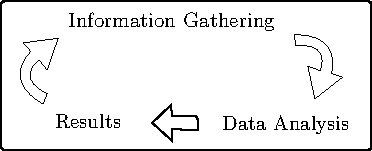
\includegraphics{images/project_cykle.pdf}
    \caption{Schematic of single iteration cycle without
      presentation.\label{fig_schematic_cycle}}
  \end{figure}

  This section will describe the considered methods of each of these phases in
  more detail.

  \subsection{Information Gathering}

    \subsubsection{Quantitative versus Qualitative}
      First There is a distinction to be made regarding qualitative and
      quantitative data. Examples of quantitative measurements are,
      \myenquote{Count of calls to the help desk} and \myenquote{Count of user
        manual accesses}\cite[p.89]{c_handbook_usability}, in other words,
      information that is easy to enumerate and describe as values. Qualitative
      data and answers are more free form and can usually not be enumerated or
      reduced to a number. Among the examples of what classifies as qualitative
      data are,
      \myenquote{Wow, I'm very, very impressed} and
      \myenquote{Can I please leave now -- keep my mony and the
        product}\cite[p.90]{c_handbook_usability}.
%    Information relevant
%    Gathering information for this project will initially

    \subsubsection{Surveys and Interviews}
      These methods can gather both qualitative and qualitative information
      and are very flexible in how they can be constructed to plumb a specific
      part of the process if it becomes extra interesting.
      This type of data gathering will be the main gathering method in the
      pilot and early prototyping stage of the project.

    \subsubsection{Prototypes and Observations}
      Past the initial prototyping and pilot stage, interaction with the current
      prototype can be analysed, and the results folded into the next iteration
      cycle. This type of observations makes it possible to measure
      quantitative data such as, time to completion of task, number of clicks
      to reach intended targets, etc. It can also become a good source for
      qualitative data, especially when encouraging participant to
      \textit{Think Aloud}\cite[p.54]{c_handbook_usability}, see below.

    \subsubsection{Thinking aloud}
      Asking test participants to produce a \textit{running commentary}
      by narrating what they are doing in real time is encouraged in order to
      get insight in why a problem exists and how a user would try to get
      around it. The method can also reveal important clues of how the user
      views and thinks about the system, which can then be compared to the
      intended design goal. It is however important to recognize that if
      precise timings are tracked, narrating should be avoided, since it
      slows down the actions of the tester\cite[p.54]{c_handbook_usability}.

  \subsection{Work Flow and Data Analysis}

    Extracting results from the acquired data and folding it back into the
    prototype and surveys will be an continuous process. The following section
    will highlight work flows and methods of analyzing the data that seem
    especially interesting.

    \subsubsection{Iteration, The Pilot and Prototyping}

      As described above, the goal is to work in a continuous state of iteration,
      shown schematically in figure \ref{fig_schematic_cycle}. In order to not
      waste valuable time by heading in the wrong direction, a pilot will be
      conducted. A pool of three to four employees will be used to provide
      feedback for the pilot phase, preferably someone from a management
      position together with a representative from each distinct discipline
      present in the team. In order to avoid biasing, these people will only be
      consulted for feedback during the pilot. Iteration on the pilot will
      continue either until the result is deemed acceptabel, nothing more of
      worth is gleaned, or the alloted time runs out.

    \subsubsection{Abandoning the Pilot}

      It is worth pointing out that the purpose of the pilot is not to generate
      ready-to-use software, surveys or other material. Rather, the pilot is
      done in order to uncover if the initial issues are the correct ones, the
      chosen methodology works, the interface framework is understandable
      enough and runs, etc. Since it is typical that the final stage of the
      prototype is built on faulty and corrected assumptions, it should not be
      used as is, rather the final assumptions should be taken into account and
      used in order to create a new basis.

    \subsubsection{Archetype Users, Personas and Scenarios}

      Archetype users or personas is a way to compress and present relevant
      information about the users of a product. A persona is an evidence-based
      user sketch that is a stand-in for a larger user group and represents
      their typical behaviour patterns and
      goals\cite[p.331]{c_handbook_usability}. \\

      Scenarios is a way to group related test-tasks and give them context. The
      scenario should be realistic with the correct motivation, match
      participants experience, retain any natural task order and not contain
      unnecessary jargon or cues to action \cite[p.182]{c_handbook_usability}.

  \subsection{Presentation of Results}

    The point of this project is to produce a result, both in the sense of
    software that tries to provide a solution to a perceived problem, and data
    points supporting or rejecting applications of usability-theory.

    \subsubsection{Intermittent}

      Presentation of intermittent results will manly include the current state
      of the interface and surveys together with any new assumptions about the
      process. This information will be delivered verbally, or at most, written
      up in a document or email and distributed to the team or project
      supervisor.

    \subsubsection{Final}

      The final presentation includes a full report and verbal presentation
      with an accompanying slide-deck. Here, the final conclusions and results
      of the project will be presented together with a summary of their
      theoretical backing.

%  In order to gather eno
%
%  There are several different
%
%  Övergripande kommer studien
%
%Thinking Aloud \cite[p.204]{c_handbook_usability}
%Simple Single-Room Setup \cite[p.101]{c_handbook_usability}
%
%  Inledningsvis kommer tre till fyra personer att väljas ut till en
%  pilotstudie för att säkerställa en korrekt riktning på testuppställningen och
%  frågor.
%
%  För att etablera ett startvärde att jämföra mot samt få en överblick, kommer
%  inledande intervjuer och enkäter om hur den nuvarande processen upplevs
%  utföras bland utvecklare och chefer. \\
%
%  [ ... ]



  %Inledningsvis behövs ett värde som den slutliga analysen kan utvärderas mot

  %Utvärdering av

  %Inledningsvis kommer intervjuer ske med de anställda för att identifiera
  %upplevda problem-områden samt skaffa sig ett initialvärde för att

\newgeometry{left=3cm, bottom=3cm}
\begin{landscape}
  \section{Time schedule} \flushleft{(Number of days from start)}
  \ \\
  \centering
  \input{tex/tidsschema.tex}
\end{landscape}
\restoregeometry

\newpage
\section{Surveys}

\begin{question}
  \qline{Alias}
  Age: \hspace{0.5cm}
    \fullmoon \ $<30$ \hh
    \fullmoon \ $31-40$ \hh
    \fullmoon \ $41-50$ \hh
    \fullmoon \ $51+$
    \ \\ \\
  \qline[Gameplay Animator]{Position}
  \qscale{I am often annoyed by the software}
  \qscale{I am often annoyed by quizzes}
  \qscale{I always know where in the process my colleges are}
  \qmline{What problems do you experience with the software}
  \qmline[4]{What positive aspects do you experience with the software}
\end{question}

\newpage
%\printbibliography[heading=bibintoc]
\printbibliography

\end{document}
